
\documentclass[12pt]{article}
\usepackage{fullpage}
\usepackage{rotating}
\usepackage{tipa}
\usepackage{gb4e}
\usepackage{amsmath}
%\usepackage{linguex}
\usepackage{enumerate}
\usepackage[sc]{mathpazo}
\usepackage{natbib}
\linespread{1.05}         % Palatino needs more leading (space between lines)
\usepackage[T1]{fontenc}

\hyphenpenalty= 7000 

\title{Software Design Document (SDD) v1.92\\  \small{ Technical Specifications \& General Information for SOEN/CompSci Interns}}
\author{}
%\date{}

\begin{document}

\maketitle{} 

\tableofcontents

\newpage
\section*{Executive Summary}
\addcontentsline{toc}{section}{Executive Summary}



\section{Introduction}


\subsection{Audience and Scope of Design}
\subsection{Terminology}
\subsection{Structure}


\section{Design Approach}

\subsection{Behaviour Driven Development (BDD)}
\subsection{Feature Tracker (Agile)}
\subsection{Chronological Growth (Blog)}
\subsection{Formal Documentation}


\section{Architecture Review}
\subsection{System Architecture}
\subsection{Instance Architecture}

\section{Composition Viewpoint}
\subsection{Data Entry Client Component}
\subsection{Import Component}
\subsection{Data Cleaning Client Component}
\subsection{ActivityFeed Client Component}
\subsection{Corpus Admin Client Component}
\subsection{Search Client Component}
\subsection{Export Client Component}
\subsection{Discoverable Pages Client Component}
\subsection{FieldMethods Admin Client Component}
\subsection{Glosser Client Component}
\subsection{Glosser Service Component}
\subsection{Lexicon Client Component}
\subsection{Grammar Client Component}
\subsection{Learn X Client Component}
\subsection{Experiment Client Component}
\subsection{Elicitation Client Component}
\subsection{Speech Service Component}
\subsection{Web Spider Service Component}
\subsection{Registration Component}
\subsection{Permissions Component}

\section{Logical Viewpoint}
\subsection{Datum Component}
\subsection{Session Component}
\subsection{Datalist Component}
\subsection{Corpus Component}
\subsection{User Component}
\subsection{Bot Component}

\section{Information Viewpoint}
\section{Interface Viewpoint}

\subsection{Supported devices and computing platforms}

\section{Interaction Viewpoint}
\subsection{Audio/Video Upload Interaction}
\subsection{Client Side Search Interaction}
\subsection{Global Search Interaction}
\subsection{Export Interaction}
\subsection{Import Interaction}
\subsection{Registration Interaction}
\subsection{Login Interaction}
\subsection{Permissions Interaction}


\section{Design Rational}


\section{Implementation Plan}

\subsection{Recommendations for web services}
\subsection{Recommendations for client modules}

\section{Summary}
\section*{References}

%\bibliography{CAML/caml2012}


\appendix
\section{Technology in Context}

\subsection{Why now: Advances in Database and Web Technologies}
\label{appendix:technology}

Since early 2010, the term \emph{NoSQL} has lead technology news. Databases can be grouped in roughly two categories, table-like (\ref{ex:whynosql}a) (also referred to as \emph{Relational}, or \emph{SQL} databases) and document-like (\ref{ex:whynosql}b) (commonly referenced in language documentation literature  simply as \emph{XML}, and in the software industry as \emph{NoSQL}).\footnote{NoSQL is actually a broad category encompasing anything which is not SQL, including documents but also interconnected web/neuron-like data strutures.} NoSQL data stores, including simple file based systems, have always existed and in fact pre-date SQL databases. Much like field linguists and language documentation standard bodies, companies who need  scalable data management such as Google \citep{Dean:2004, Dean:2008}  Adobe \citep{Lehene:2010:Online} Facebook \citep{Borthakur:2011}  and LinkedIn \citep{Sumbaly:2013} actively resist SQL (frequently proprietary) data storage solutions  (\ref{ex:databasetrends}a) and seek open source NoSQL solutions (\ref{ex:databasetrends}b). 

By April 2012 when LingSync began, NoSQL databases had matured to the extent that they were well understood, and deployed at large scale. 
Using an existing mature NoSQL database solution has greatly reduced the novel code needed to build LingSync, meaning we were able to focus our efforts on building usable user interfaces, and integrating our favourite field linguistics tools as modules and plugins to help automate the data entry process. 




\begin{exe}

  \ex   Illustration of the storage requirements vs self-documenting ability of NoSQL
  \centering
    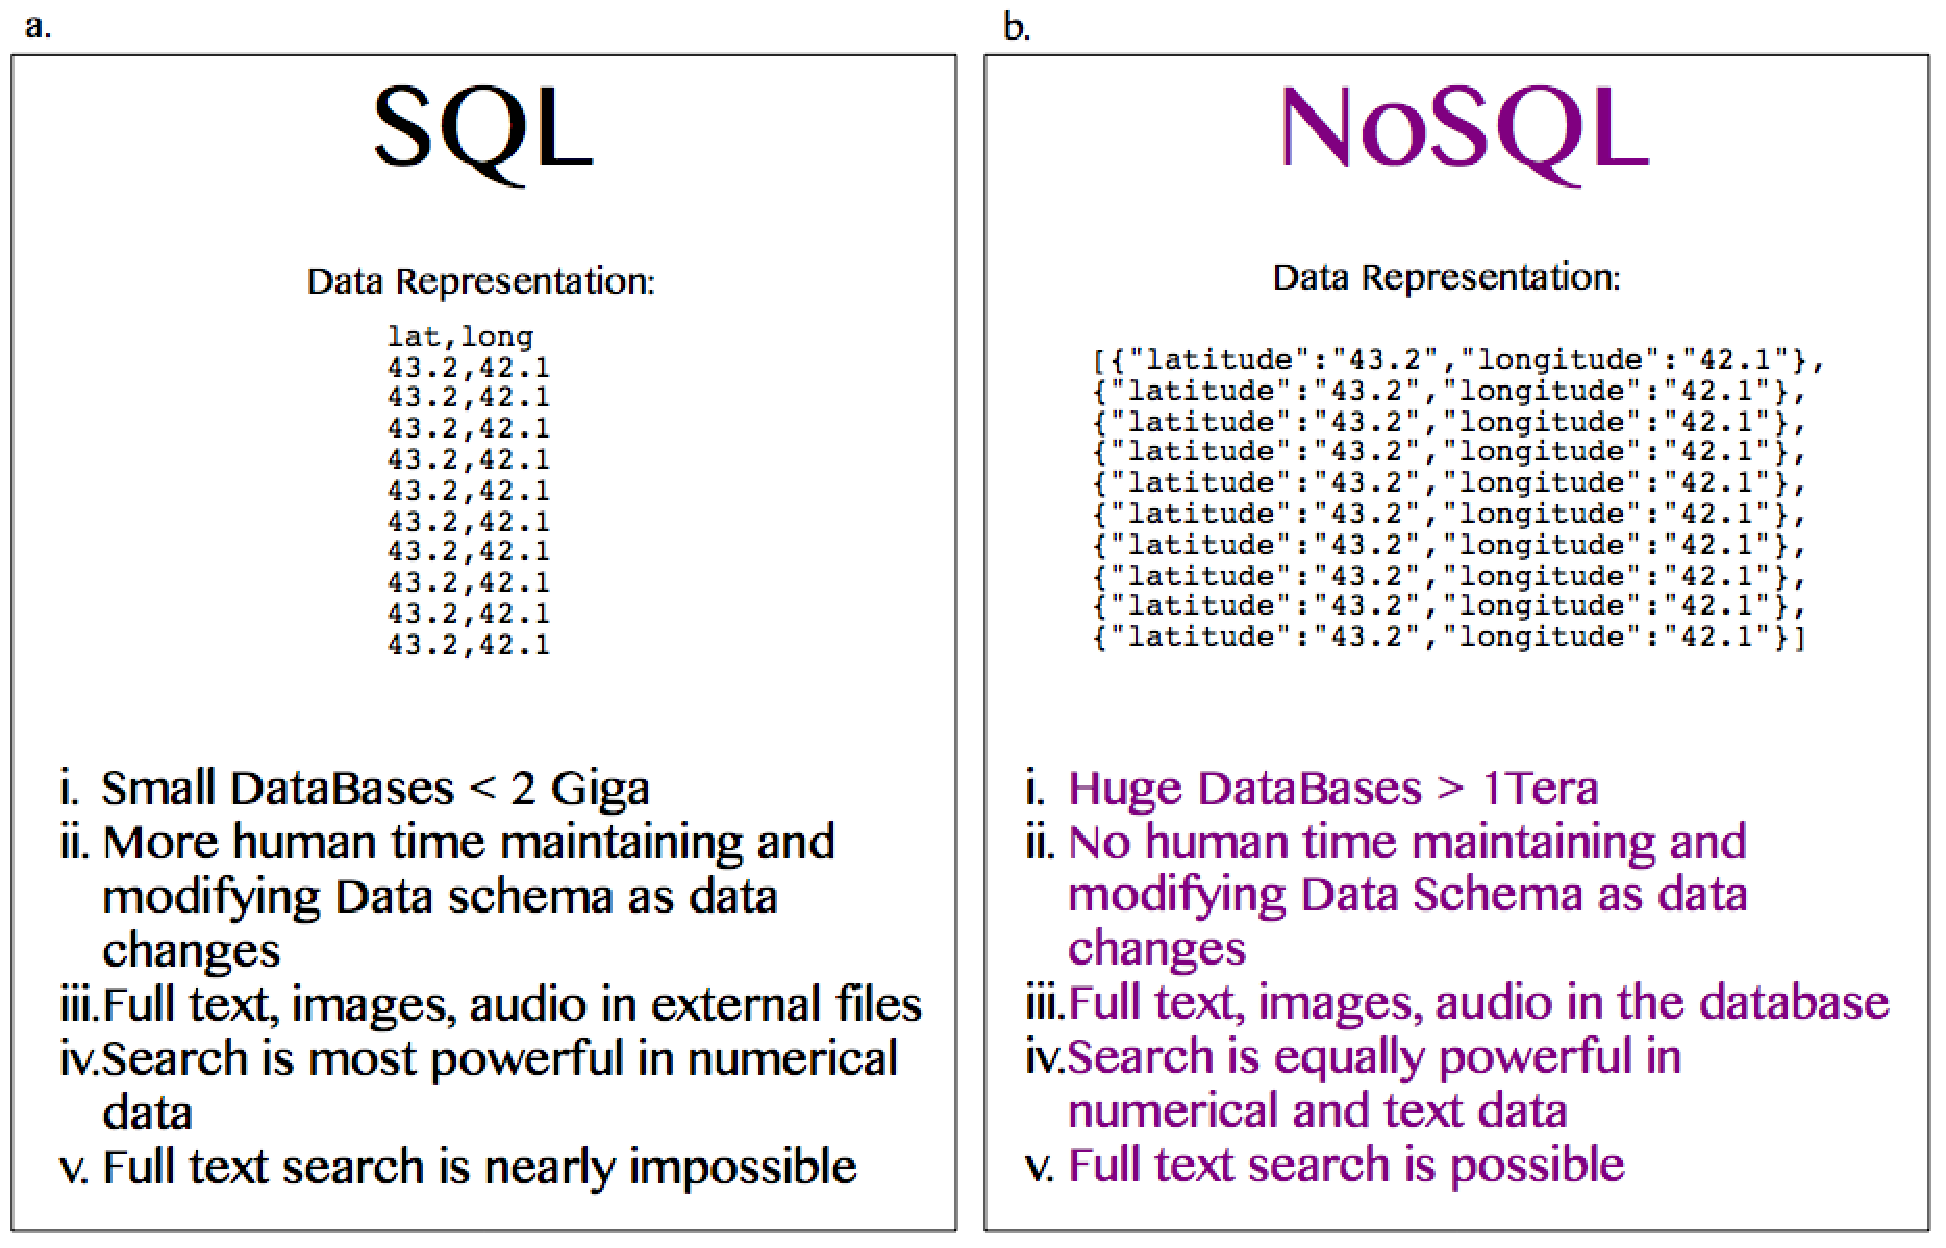
\includegraphics[width=0.8\textwidth]{figures/whynosql}

\label{ex:whynosql}
\end{exe}


\begin{exe}

  \ex   Currently human resources are very expensive while hardware is inexpensive, resulting in a growing popularity of NoSQL databases including what is under LingSync (CouchDB)
  \centering
    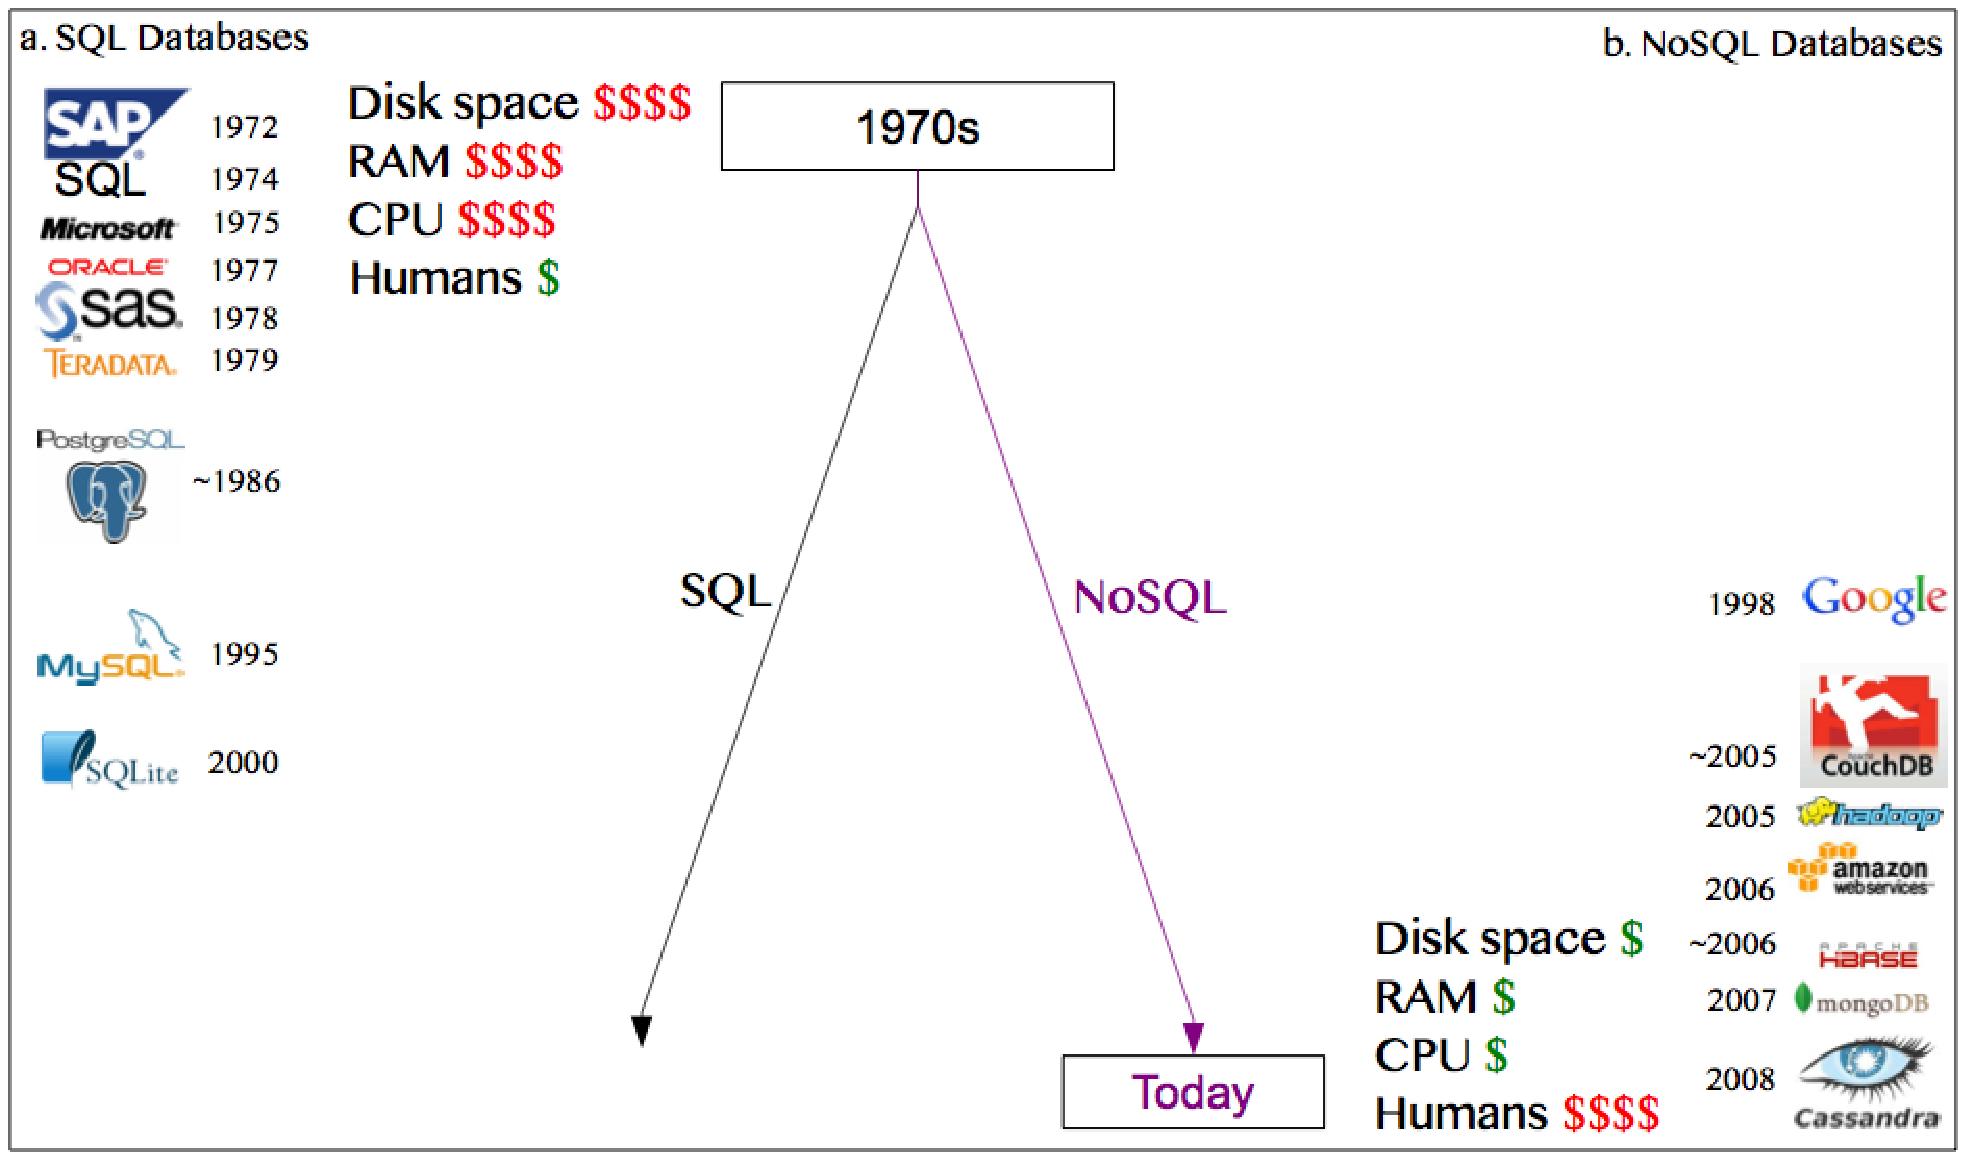
\includegraphics[width=0.8\textwidth]{figures/databasetrends}

\label{ex:databasetrends}
\end{exe}


In June 2012, only one month before we launched the project at CAML, it became possible to build a web app which also worked offline. 
%\footnote{To develop LingSync we had been using a developer edition of Chrome which was two months before normal Chrome.}
 In April 2013 CouchDB added CORS (Cross-Origin Resource Sharing) support,  permitting what are called `mashups' essentially the ability for one to build  independent apps which interfaces with LingSync data securely in realtime, with no additional infrastructure. 

Prior to 2011 there is one other aspect of LingSync which was not possible: only one programming language is used throughout LingSync. The web services are written in JavaScript, the user interface is written in JavaScript, and even the database queries are written in JavaScript. JavaScript has a very simple yet consistent syntax, and only a handful of data types, meaning that research assistants can learn to script in less than one week, and even design and complete their own components in one semester. JavaScript has only recently become a popular programming language, and as such there are a wealth of beginner friendly video screencasts and tutorials which are targeted at non-programmers. Prior to 2011 research assistants frequently learned Python, Bash, and Unix utilities to help clean and transform data,  in addition of course to \LaTeX  and/or Praat. Unlike professional fieldwork, research is unknown, no software can plan everything a research team might wish to do with their data.  As most research budgets are dedicated to funding students, and a growing number of linguistics students come to a department with a basic knowledge of web programming, a viable solution is ask research assistants to manipulate data in batches via scripts. Without a bit of scripting, research assistance are relegated to tasks of monotonous repetition which must be performed in a consistent manner. Training research assistants to script data manipulation not only saves time, but also permits labs to pass on technical knowledge to future lab members, rather than outsourcing  data management to external consultants or computer science students who have largely been trained on SQL best practices which contradict the best practices  needed for smooth data management of the NoSQL data inherent in fieldwork. \cite{Thieberger:2012} also advocates in-house learning, ``there is a need for data management skills to be developed among linguistic scholars so that our relatively small collections can be maintained.''% \citep[p.133]{}   

%It is also worth noting the ability of primary video and audio data to reside in the same system as text data has matured and is as of 2012 is mature enough on all laptops in the form of HTML5 audio and video. \citep{Pfeiffer:2010}.
 
\section{Data Models}

\subsection{Datum}
\label{appendix:datumjson}

\begin{verbatim}
{
   "_id": "89bc4d7dcc2b1fc9a7bb0f4f474a7fb4",
   "_rev": "7-0d53714bc3b67681892fa0791cbebac3",
   "audioVideo": [],
   "comments": [
       {
           "text": "Hi\nJust a quick note to say that I automatically cleaned this datum. \n\nChanges:\n *  quote encoding problems `We feel like yelling at the children.\" -> We feel like yelling at the children.\n\nExplanation: I was asked by lingllama to come by and standardize quotes today. According to his corpus' convention, we don't need quotes in the translation field.",
           "username": "quotecleaningbot",
           "timestamp": 1389642361952,
           "gravatar": "968b8e7fb72b5ffe2915256c28a9414c",
           "timestampModified": 1389642361952
       }
   ],
   "dateEntered": "\"2013-03-17T23:07:42.760Z\"",
   "dateModified": "\"2013-12-02T20:19:17.321Z\"",
   "datumFields": [
       {
           "label": "judgement",
           "value": "*",
           "mask": "*",
           "encrypted": "",
           "shouldBeEncrypted": "",
           "help": "Grammaticality/acceptability judgement (*,#,?, etc). Leaving it blank can mean grammatical/acceptable, or you can choose a new symbol for this meaning.",
           "size": "3",
           "showToUserTypes": "linguist",
           "userchooseable": "disabled"
       },
       {
           "label": "utterance",
           "value": "Erqekunata noqayku qaparinaywanku.",
           "mask": "Erqekunata noqayku qaparinaywanku.",
           "encrypted": "",
           "shouldBeEncrypted": "checked",
           "help": "Unparsed utterance in the language, in orthography or transcription. Line 1 in your LaTeXed examples for handouts. Sample entry: amigas",
           "showToUserTypes": "all",
           "userchooseable": "disabled"
       },
       {
           "label": "morphemes",
           "value": "Erqe-kuna-ta noqa-yku qapari-nay-wanku",
           "mask": "Erqe-kuna-ta noqa-yku qapari-nay-wanku",
           "encrypted": "",
           "shouldBeEncrypted": "checked",
           "help": "Morpheme-segmented utterance in the language. Used by the system to help generate glosses (below). Can optionally appear below (or instead of) the first line in your LaTeXed examples. Sample entry: amig-a-s",
           "showToUserTypes": "linguist",
           "userchooseable": "disabled",
           "alternates": [
               "Erqekuna-ta noqayku qapari-nay-wanku.",
               "Erqe-kuna-ta noqayku qapari-nay-wanku.",
               "Erqekunata noqayku qaparinaywanku."
           ]
       },
       {
           "label": "gloss",
           "value": "child-PL-ACC 1PL.ex yell-DES-3PL.1PLexOM",
           "mask": "child-PL-ACC 1PL.ex yell-DES-3PL.1PLexOM",
           "encrypted": "",
           "shouldBeEncrypted": "checked",
           "help": "Metalanguage glosses of each individual morpheme (above). Used by the system to help gloss, in combination with morphemes (above). It is Line 2 in your LaTeXed examples. We recommend Leipzig conventions (. for fusional morphemes, - for morpheme boundaries etc)  Sample entry: friend-fem-pl",
           "showToUserTypes": "linguist",
           "userchooseable": "disabled",
           "alternates": [
               "?-ACC ? yell-DES-?",
               "child-PL-ACC ? yell-DES-?",
               "Erqe-kuna-ta noqayku qapari-nay-wanku.",
               "Erqekuna-ta noqayku qapari-nay-wanku."
           ]
       },
       {
           "label": "syntacticCategory",
           "value": "",
           "mask": "",
           "encrypted": "",
           "shouldBeEncrypted": "checked",
           "help": "This optional field is used by the machine to help with search and data cleaning, in combination with morphemes and gloss (above). If you want to use it, you can choose to use any sort of syntactic category tagging you wish. It could be very theoretical like Distributed Morphology (Sample entry: ?-GEN-NUM), or very a-theroretical like the Penn Tree Bank Tag Set. (Sample entry: NNS) http://www.ims.uni-stuttgart.de/projekte/CorpusWorkbench/CQP-HTMLDemo/PennTreebankTS.html",
           "showToUserTypes": "machine",
           "userchooseable": "disabled"
       },
       {
           "label": "translation",
           "value": "We feel like yelling at the children.",
           "mask": "We feel like yelling at the children.",
           "encrypted": "",
           "shouldBeEncrypted": "checked",
           "help": "Free translation into whichever language your team is comfortable with (e.g. English, Spanish, etc). You can also add additional custom fields for one or more additional translation languages and choose which of those you want to export with the data each time. Line 3 in your LaTeXed examples. Sample entry: (female) friends",
           "showToUserTypes": "all",
           "userchooseable": "disabled"
       },
       {
           "label": "tags",
           "value": "Impulsative, Person, Agreement",
           "mask": "Impulsative, Person, Agreement",
           "encrypted": "",
           "shouldBeEncrypted": "",
           "help": "Tags for constructions or other info that you might want to use to categorize your data.",
           "showToUserTypes": "all",
           "userchooseable": "disabled"
       },
       {
           "label": "validationStatus",
           "value": "CheckedWithSeberina",
           "mask": "CheckedWithSeberina",
           "encrypted": "",
           "shouldBeEncrypted": "",
           "help": "For example: To be checked with a language consultant, Checked with Sebrina, Deleted etc...",
           "showToUserTypes": "all",
           "userchooseable": "disabled"
       },
       {
           "label": "dateElicited",
           "value": "5/7/2010",
           "mask": "5/7/2010",
           "encrypted": "",
           "shouldBeEncrypted": "checked",
           "help": "This field came from file import ",
           "userchooseable": ""
       },
       {
           "label": "notesFromOldDB",
           "value": "backwards agreement",
           "mask": "backwards agreement",
           "encrypted": "",
           "shouldBeEncrypted": "checked",
           "help": "This field came from file import ",
           "userchooseable": ""
       },
       {
           "label": "dialect",
           "value": "Cusco Quechua",
           "mask": "Cusco Quechua",
           "encrypted": "",
           "shouldBeEncrypted": "checked",
           "help": "This field came from file import ",
           "userchooseable": ""
       },
       {
           "label": "syntacticTreeLatex",
           "value": "",
           "mask": "",
           "encrypted": "",
           "shouldBeEncrypted": "",
           "help": "This optional field is used by the machine to make LaTeX trees and help with search and data cleaning, in combination with morphemes and gloss (above). If you want to use it, you can choose to use any sort of LaTeX Tree package (we use QTree by default) Sample entry: Tree [.S NP VP ]",
           "showToUserTypes": "machine",
           "userchooseable": "disabled"
       },
       {
           "label": "enteredByUser",
           "value": "",
           "mask": "",
           "encrypted": "",
           "shouldBeEncrypted": "",
           "help": "The user who originally entered the datum",
           "showToUserTypes": "all",
           "readonly": true,
           "userchooseable": "disabled"
       },
       {
           "label": "modifiedByUser",
           "value": "public",
           "mask": "public",
           "encrypted": "",
           "shouldBeEncrypted": "",
           "help": "An array of users who modified the datum",
           "showToUserTypes": "all",
           "readonly": true,
           "users": [
               {
                   "username": "public",
                   "gravatar": "968b8e7fb72b5ffe2915256c28a9414c",
                   "firstname": "",
                   "lastname": ""
               }
           ],
           "userchooseable": "disabled"
       }
   ],
   "pouchname": "lingllama-communitycorpus",
   "session": {
       "sessionFields": [
           {
               "label": "goal",
               "value": "This data was collected by ME Cathcart for her dissertation \"Impulsatives: The syntax and semantics of involuntary desire\" for more of her data: https://github.com/mecathcart/Impulsatives",
               "mask": "This data was collected by ME Cathcart for her dissertation \"Impulsatives: The syntax and semantics of involuntary desire\" for more of her data: https://github.com/mecathcart/Impulsatives",
               "encrypted": "",
               "shouldBeEncrypted": "",
               "help": "This describes the goals of the session.",
               "userchooseable": "disabled"
           },
           {
               "label": "consultants",
               "value": "Lucia, Ricardo, Seberina",
               "mask": "Lucia, Ricardo, Seberina",
               "encrypted": "",
               "shouldBeEncrypted": "",
               "help": "Example from DataOne: Format conventions: use uppercase ,Codes for missing values: unknown",
               "userchooseable": "disabled"
           },
           {
               "label": "dialect",
               "value": "",
               "mask": "",
               "encrypted": "",
               "shouldBeEncrypted": "",
               "help": "You can use this field to be as precise as you would like about the dialect of this session.",
               "userchooseable": "disabled"
           },
           {
               "label": "language",
               "value": "",
               "mask": "",
               "encrypted": "",
               "shouldBeEncrypted": "",
               "help": "This is the langauge (or language family) if you would like to use it.",
               "userchooseable": "disabled"
           },
           {
               "label": "dateElicited",
               "value": "Summer 2010",
               "mask": "Summer 2010",
               "encrypted": "",
               "shouldBeEncrypted": "",
               "help": "This is the date in which the session took place.",
               "userchooseable": "disabled"
           },
           {
               "label": "user",
               "value": "",
               "mask": "",
               "encrypted": "",
               "shouldBeEncrypted": "",
               "help": "Example from DataOne: Format conventions: use uppercase ,Codes for missing values: unknown",
               "userchooseable": "disabled"
           },
           {
               "label": "dateSEntered",
               "value": "",
               "mask": "",
               "encrypted": "",
               "shouldBeEncrypted": "",
               "help": "This is the date in which the session was entered.",
               "userchooseable": "disabled"
           }
       ],
       "pouchname": "lingllama-communitycorpus",
       "comments": [
       ],
       "dateCreated": "\"2013-03-17T23:07:34.194Z\"",
       "dateModified": "\"2013-03-17T23:07:34.194Z\"",
       "timestamp": 1363561654194,
       "_id": "89bc4d7dcc2b1fc9a7bb0f4f474415e4",
       "_rev": "1-701f44686ae45a27d4e5a08ed6c26dc8"
   },
   "timestamp": 1386015557322,
   "jsonType": "Datum",
   "collection": "datums"
}
\end{verbatim}


\section{Module Implementations}

In this section we discuss in detail the timeline and budget for each of the modules that make up the LingSync application. The modules are grouped into core modules and dream modules which will be made when the budget becomes available. 

\label{sec:modules}
\subsection{Core Modules}

The project has three core modules which must be developed prior to additional modules. These are the {\it collaboration, corpus} and {\it lexicon} modules, briefly outlined in terms of functionality and timeline in the following sections.  Implementation of the three core modules began on April 20th 2012. The three core modules will be launched on August 1st at CAML in Patzun Guatemala. We estimate the three core modules and the software architecture to take 9.2 weeks to complete with three software developers,  and cost roughly \$23,800 before taxes. We will have its final time and costs on August 3rd 2012.


\newpage
\subsubsection{Collaboration Module}
The collaboration module shown in Table~\ref{table-collaboration}  deals with users, teams, permissions, user authentication,  as well as allowing users to see changes, modifications, and data verification in the form of an ``Activity Feed.'' An activity feed is a common design pattern which allows users to learn form other users how to use the software, what are popular functions other users are completing in addition to being a central location to update oneself on the activity in the corpus. The system will have special users called ``bot'' which are scripts or programs which power users can write in Javascript which will crawl their corpus and clean/automate batch actions.

We estimate the total cost of the collaboration module to be around \$5,700 before taxes. The implementation of the collaboration module was begun on April 20th 2012, and finished on August 1st 2012, with the exception of Team Feed and Team Preference Widgets. 
%User/Consultant/Team tests are not done either. 
\begin{table}[h]
\begin{center}
  \begin{tabular}{ | lcl | }
\hline
Iteration&  Hours&  Technology  \\
\hline
Software Architecture Design& 20& Software Engineering  \\ 
Collaboration API on central server&  30& Software Engineering\\ 
Users Model&  15& Javascript  \\ 
consultant Model& 15& Javascript  \\ 
Team Model& 15& Javascript  \\ 
Bot Model&  15& Javascript  \\ 
User Activity Model&  8&  Javascript  \\ 
Team Feed Widget& 25& HTML5 \\ 
User list item Widget&  16& HTML5 \\ 
Team Preferences Widget&  8&  HTML5 \\ 
User Profile Widget&  8&  HTML5 \\ 
User Tests& 30& Javascript \\ 
Consultant Tests& 30& Javascript  \\ 
Team Tests& 30& Javascript  \\ 
Android Deployment& 15& Java  \\ 
Chrome Extension Deployment&  20& Javascript \\ 
Heroku Deployment&  5&  Integration \\ 
%\# of weeks with 3 full time personnel&  2.5416666667& \\ 
\hline
  \end{tabular}
  \caption{The Collaboration Module is used to permit collaboration with teams and users. }
\label{table-collaboration}
  \end{center}
\end{table}


\newpage
\subsubsection{Corpus Module}
The corpus module shown in Table~\ref{table-corpus} deals with storing confidential data in the AES US Federal encryption standard, replicating the corpus locally on the  users' computers, as well as on a central server hosted either in the cloud, or on a linguistic department's server. The corpus module contains all of the core logic, including data fields, session fields, as well as data lists which are used to curate lists of data for handouts or publication either in linguistic articles or as web widgets embedded in external websites such as linguistic department blogs, or project pages. The corpus module is also where search of datum is implemented. 

We estimate the total cost of the corpus module to be around \$9,200 before taxes. The implementation of the corpus module was begun on April 20th 2012, and finished on August 1st 2012, with the exception of Corpus diff Widget.
\begin{table}[htbp]
\begin{center}
  \begin{tabular}{ | lcl | }
\hline

Iteration&  Hours&  Technology  \\
\hline
Software Architecture Design& 20& Software Engineering  \\ 
Corpus API on corpus server&  20& Software Engineering\\ 
Corpus Model& 8&  Javascript  \\ 
Session Model&  8&  Javascript  \\ 
Datum Model&  8&  Javascript  \\ 
Datum status model& 8&  Javascript  \\ 
DataList Model& 8&  Javascript  \\ 
Confidential datum encrypter& 16& Javascript  \\ 
Audio upload and play logic&  8&  Javascript  \\ 
Corpus DB  implementation on Android& 20& Java  \\ 
Corpus DB  implementation on Chrome&  20& Javascript  \\ 
Corpus DB  implementation on Node.js& 20& Javascript \\ 
Corpus versioning Logic&  25& Javascript  \\ 
Corpus Preferences Widget&  6&  HTML5 \\ 
Session Preferences Widget& 6&  HTML5 \\ 
Datum Preferences Widget& 20& HTML5 \\ 
Datum Status Preferences Widget&  16& HTML5 \\ 
DataList Preferences Widget&  6&  HTML5 \\ 
Corpus sync logic&  10&  Javascript \\ 
Corpus diff Widget (to show before sync)& 10&  HTML5 \\ 
Insert Unicode Character Widget&  10&  HTML5 \\ 
Corpus Details Widget&  6&  HTML5 \\
Session Details Widget& 6&  HTML5 \\  
Datum Details Widget& 20&  Javascript \\ 
DataList Widget&  30&  Javascript \\ 
Global Search logic&  30&  Javascript \\ 
Power Search logic& 80&  Javascript \\ 
Corpus Tests& 5&  Javascript \\ 
Session Tests&  10&  Javascript \\ 
Datum Tests&  10&  Javascript \\ 
Datum Status Tests& 10&  Javascript \\ 
DataList Tests& 20&  Javascript \\ 
Heroku Deployment&  5&  Integration \\ 
\hline
  \end{tabular}
 \caption{The Corpus Module is used to sync, share, edit, tag, categorize and open data. }
\label{table-corpus}
  \end{center}
\end{table}
%# of weeks with 3 full time personnel  4.20833333333333


\newpage
\subsubsection{Lexicon Module}

The lexicon module show in Table~\ref{table-lexicon} is used for search. It is loosely modeled after a mental lexicon, in a network of morphemes, allomorphs, orthographie(s), glosses and translations.  It is not a dictionary but rather a connected graph similar to theoretical models of mental lexicons (for a dictionary see the Dictionary Module in \S~\ref{module-dictionary}). As a connected graph it is the most useful structure to index datum and search for datum real time while data entry is happening. 
%One requested use-case was to have the search open for a particular morpheme/category and have datum which are entered show up in the search results. 

We estimate the total cost of the lexicon module to be around \$7,300 before taxes. The implementation of the lexicon module was begun on April 20th 2012. We will know its final costs on August 3rd 2012.

\begin{table}[htbp]
\begin{center}
  \begin{tabular}{ | lcl | }
\hline

Iteration&  Hours&  Technology  \\
\hline
Software Architecture Design& 20& Software Engineering  \\ 
Lexicon API on Lexicon server&  20& Software Engineering\\ 
Lexicon Model&  6&  Javascript  \\ 
Morpheme Model& 6&  Javascript  \\ 
Allomorph Model&  6&  Javascript  \\ 
Gloss Model&  6&  Javascript  \\ 
Orthography Model&  16& Javascript  \\ 
Lexicon DB  implementation on Android&  20& Java  \\ 
Lexicon DB  implementation on Chrome& 20& Javascript  \\ 
Lexicon DB  implementation on Node.js&  20& Javascript \\ 
Lexicon versioning Logic& 10& Javascript  \\ 
Lexicon Preferences Widget& 6&  HTML5 \\ 
Morpheme Tests& 6&  Javascript  \\ 
Allomorph Tests&  6&  Javascript \\ 
Gloss Tests&  6&  Javascript  \\ 
Orthography Tests&  8&  Javascript \\ 
Lexicon Analysis Widget&  10&  HTML5 \\ 
Lexicon sync logic& 10&  Javascript \\ 
Lexicon diff Widget (to show before sync)&  10&  HTML5 \\ 
Lexicon Details Widget& 6&  HTML5 \\
Lexicon Tests&  12&  Javascript \\  
Heroku Deployment&  5&  Integration \\ 
\hline
  \end{tabular}
 \caption{The Lexicon Module is used to house, and read lexicon entries to be used for the glosser.}
 \label{table-lexicon}
  \end{center}
  

\end{table}
%# of weeks with 3 full time personnel  1.95833333333333

\subsection{``Dream'' Modules}

The "dream" modules allow for more features that will save researchers time in their data entry and data analysis, but which are not necessary for simply entering and transcribing data. These modules are on hold until budget becomes available.


\subsubsection{Language Learning Module}
The language learning module shown in Table ~\ref{tab:langlearn} enables researchers and language teachers to create language learning aids from the data in existing corpora and from the data newly collected for the purpose of language learning. The learning aids aim to help language learners improve their listening and speaking skills. The orthographic lines (i.e. utterance and morpheme lines) and the attached audio or video recordings of a datum are taken as materials to create a lesson. 


The prototype of the language learning module was begun on September 13th 2012.

\begin{table}[htbp]
\begin{center}
  \begin{tabular}{ | lcl | }
\hline
Iteration &  Hours &  Technology  \\
\hline
-- Prototype && \\ 
Software Architecture Design & 55 & Software Engineering \\
Lesson Datum Model & 15  & Javascript \\
Lesson Datum Listen and Repeat View & 20  & Javascript \\
XML import logic  & 6 & Javascript \\ 
Datum to Lesson logic  & 6  & Map Reduce \\ 
DataList to Unit logic  & 6  & Map Reduce \\ 
Corpus to Language Learning logic  &  10  & Map Reduce \\ 
Main Manu Dashboard  & 6  & HTML \\ 
Student LIsten and Repeat Dashboard  & 10  & HTML \\ 
Student Instructions View  & 6  & Javascript \\ 
Audio Visualization View  & 30  & Javascript \\ 
Audio Play/Record View  & 10  & Javascript \\ 
Audio Text Time Alignment logic  & 20  & Javascript \\ 
Audio Record Android logic  &  6  & Java \\ 
Android Packaging  & 15  & Java \\ 
% # of weeks with 1 full-time personnel supervising 2 interns 4.775 
\hline 
Software Architecture Design & 40 & Software Engineering  \\ 
Teacher User Model  &  10 &  Javascript \\ 
Teacher User View  &  40  & Javascript \\ 
Language Learning Corpus  &  10 &  Javascript \\ 
Language Learning Corpus View  &  40  & Javascript \\ 
Language Learning Corpus Dashboard  &  10  & HTML \\ 
Student User Model  &  30  & Javascript \\ 
Student User View  &  60  & Javascript \\ 
Datum Shadowing Lesson Model  & 10 & Javascript \\ 
Datum Shadowing Lesson View  &  10  &  Javascript \\ 
Student Shadowing Lesson Dashboard &  40 & HTML \\ 
Datum Quiz Multiple Choice Model  & 20  & Javascript \\ 
Datum Quiz Multiple Choice View  &  20  & Javascript \\ 
Student Quiz Dashboard  & 120  & HTML \\ 
Datum Prompted Production Model  & 20  & Javascript \\ 
Datum Prompted Production View  & 20  & Javascript \\ 
Student Prompted Productions Dashboard  &  40  & HTML \\ 
Feedback Comment Model  & 10  & Javascript \\ 
Feedback Comment View  & 40  & Javascript \\ 
Comment Teacher Feedback logic & 6  & Map Reduce \\ 
Audio import to Multiple Utterances logic   & 60  & Praat \& Javascript \\ 
Audio File Server  & 140  & Node \\ 
% # of weeks with 1 full-time personnel 19.4 
\hline
  \end{tabular}
 \caption{The Language Learning Module enables to use data in the database to create lessons for language learners.  }
  \label{tab:langlearn}
  \end{center}
\end{table}



\subsubsection{Phonological Search Module}
The phonological search module shown in Table~\ref{tab:phono} is used to search for phonological features in context. It consists of a phonology ontology (a general purpose feature geometry/articulatory feature ontology, or a customized ontology created by the users for their language of interest) which lets the user search for potential minimal pairs or phonological features in context to verify with consultants or to prepare psycholinguistic experiments. The phonological search module is used by the {\it  phonetic aligner} module to generate a ``dictionary.txt'' file containing orthography and phones which is used by the phonetic aligner module.

We estimate the cost of the phonological search module to be roughly \$2,200 before taxes. The Phonological search, or the phonetic aligner module is currently schedule to begin in September 2012, we haven't yet decided which is a priority.

\begin{table}[htbp]
\begin{center}
  \begin{tabular}{ | lcl | }
\hline
Iteration&  Hours&  Technology  \\
\hline
Phonology Ontology for phonological search& 60& Java  \\ 
Lexicon Visualization Widget& 40& Javascript  \\ 
Lexicon Editing Widget& 20& Javascript  \\ 
\hline
  \end{tabular}
 \caption{This module is a subportion of the Lexicon Module.}
  \label{tab:phono}
  \end{center}
\end{table}
%# of weeks with 1 full time personnel  3


\newpage
\subsubsection{Phonetic Aligner Module}
The phonetic aligner module show in Table~\ref{tab:aligner} makes it possible to use attached audio recordings and the orthographic/utterance lines of datum to create a dictionary unique to the corpus' language, and to run the ProsodyLab Aligner, a machine learning algorithm which uses Hidden Markov Models to predict boundaries between phones and creates a Praat TextGrid with estimated phone boundaries, saving hours of boundary tagging. We also have factored in a bit of sound editing to facilitate the process of creating audio files which correspond closely to the utterance line in the datum's fields. 


We estimate the cost of the phonetic aligner module to be roughly \$9,800 before taxes. The phonetic aligner or the phonological search module is currently scheduled to begin in September 2012, we haven't yet decided which is a priority.
\begin{table}[htbp]
\begin{center}
  \begin{tabular}{ | lcl | }
\hline

Iteration&  Hours&  Technology  \\
\hline
Software Architecture Design& 10& Software Engineering  \\ 
Aligner API on Lexicon server&  10& Software Engineering\\ 
Dictionary Model& 15& Javascript  \\ 
Aligner DB implementation&  80& Integration \\ 
Aligner Machine Learning Integration& 80& Java  \\ 
Aligner Preferences Widget& 8&  HTML5 \\ 
Audio Waveform Visualization logic& 30& Javascript  \\ 
Audio Spectrogram Visualization logic&  ?&  Javascript \\ 
Transcription User Interface& 80& HTML5 \\ 
TextGrid export&  20&  Javascript \\ 
Dialect Profile Widget&          8&  HTML5 \\ 
Orthography Tests&  30&  Javascript \\ 
Training Tests& 30& Java  \\ 
Heroku Deployment&  5&  Integration \\ 
\hline
  \end{tabular}
  \caption{The Aligner Module is used to create TextGrids from the orthography and the audio files, used for prosody and phonetic analysis.}
  \label{tab:aligner}
  \end{center}
\end{table}
%# of weeks with 1 full time personnel  10.15



\newpage
\subsubsection{Dictionary Module}

The dictionary module shown in Table~\ref{tab:dictionary}is used to crawl the corpus to gather citations and examples to build a Wiktionary dictionary for the corpus' language, as required by some grants which focus on endangered/minority languages. The dictionary module is quite complex and the central component of many online fieldlinguistics databases.   

We estimate the dictionary module to cost roughly \$ 18,800 before taxes. The dictionary module is not currently scheduled until we have more users who require its functionality.
\label{module-dictionary}
\begin{table}[htbp]
\begin{center}
  \begin{tabular}{ | lcl | }
\hline

Iteration&  Hours&  Technology  \\
\hline
Software Architecture Design& 40& Software Engineering  \\ 
Dictionary API on Lexicon server& 30& Software Engineering\\ 
Semantic Model& 60& Javascript  \\ 
Syntactic Model&  60& Javascript  \\ 
Citation Model& 60& Javascript  \\ 
Synonyms Model& 60& Javascript  \\ 
Dictionary DB implementation& 80& Integration \\ 
Dictionary Training Logic&  80& Java  \\ 
Web Spider Training Logic&  100&  Java  \\ 
Dictionary Preferences Widget&  8&  HTML5 \\ 
Dictionary WordNet Analysis Widget& 120&  HTML6 \\ 
Dialect Profile Widget& 8&  HTML5 \\ 
Semantic Tests& 30& Javascript  \\ 
Syntactic Tests&  30&  Javascript \\ 
Citation Tests&          30&  Javascript \\ 
Synonyms Tests& 30&  Javascript \\ 
Spider Tests& 30& Java \\ 
Training Tests& 30& Java  \\ 
Heroku Deployment&  5&  Integration \\ 
\hline
  \end{tabular}
 \caption{The Dictionary Module is used to share the lexicon in the form of a WordNet/Wiktionary dictionary with the language community as required by some grants.}
  \label{tab:dictionary}
  \end{center}
\end{table}
%# of weeks with 1 full time personnel  22.275


\newpage
\subsubsection{Glosser Module}
The glosser module show in Table~\ref{tab:glosser} is designed to make the app ``smarter'' and to reduce the amount of time spent entering predictable information such as glosses. The glosser can use any existing morphological analysis tool to break down the utterance/orthography line  into a probable morphological segmentation using known morphemes in the lexicon, and enters a probable gloss for the morphemes in the glossing line. The glosser module is designed to reduce redundant data entry, not to provide accurate glosses. It is of course crucial that predicted morpheme segmentation and glosses be corrected by users, particularly in languages where morphemes are ambiguous, or where morphemes are short and hence there are more ambiguous morpheme segmentations for words. 


We estimate the glosser module to cost roughly \$17,800. The glosser module is not currently scheduled until we have more users who require its functionality.
\begin{table}[htbp]
\begin{center}
  \begin{tabular}{ | lcl | }
\hline

Iteration&  Hours&  Technology  \\
\hline
Software Architecture Design& 40& Software Engineering  \\ 
Glosser API on Lexicon server&  30& Software Engineering\\ 
Morpheme Model& 15& Javascript  \\ 
Allomorph Model&  15& Javascript  \\ 
Gloss Model&  15& Javascript  \\ 
Orthography Model&  30& Javascript  \\ 
Glosser DB implementation&  80& Integration \\ 
Glosser Prediction Logic& 80& Java  \\ 
Glosser Machine Learning Logic& 80& Java  \\ 
Glosser Training Logic& 80& Java  \\ 
Web Spider Training Logic&  80& Java  \\ 
Glosser Preferences Widget& 8&  HTML5 \\ 
Morphological Analysis Widget&  40& HTML6 \\ 
Dialect Profile Widget& 8&  HTML5 \\ 
Morpheme Tests& 30& Javascript  \\ 
Allomorph Tests&  30&  Javascript \\ 
Gloss Tests&           30&  Javascript \\ 
Orthography Tests&  30&  Javascript \\ 
Spider Tests& 30& Java \\ 
Training Tests& 30& Java  \\ 
Heroku Deployment&  5&  Integration \\ 
\hline
  \end{tabular}
   \caption{The Glosser Module is used to automatically gloss datum, smarter than the standard lexicon.}
  \label{tab:glosser}
  \end{center}
\end{table}
%# of weeks with 1 full time personnel  19.65

\subsubsection{Web Spider Module}

The Web Spider module shown in Table~\ref{table-spider} is a non-crucial module which allows researchers with limited access to consultants to gather data using blogs or forums. The web spider also provides an additional source of context to assist consultants in providing grammaticality judgements, as well as additional contexts where morphemes appear. For example, ``ke'' is largely considered a postposition by Urdu-consultants with explicit knowledge, however it is often produced as other functional morphemes in everyday spoken contexts. Blog/forum data can be used to discover these additional contexts.


The Web Spider module is currently not a scheduled module.  It will not become a priority until we have more users who require its functionality.

\begin{table}[htbp]

\begin{center}
  \begin{tabular}{ | lcl | }
\hline
Iteration&  Hours&  Technology  \\
\hline
Corpus Visualization Widget&  40& HTML5 \\ 
Web Spider Training Logic&  60& Java  \\ 
\hline
  \end{tabular}
  \caption{The Spider module allows for collection and annotation of E-Language data.}
\label{table-spider}
  \end{center}
\end{table}
%# of weeks with 1 full time personnel  2.5



\newpage
\subsubsection{User Support \& Maintenance}

The user support  \& maintenance module shown in Table~\ref{tab:support} includes general support, new features, upgrades, and maintenance. User support includes answering user's emails, helping system administrators install the app and its various server apps on their department server, creating video tutorials, screen casts and sample data to help users figure out the application and begin using it immediately, as well as discover some of its advanced/unexpected features. 

We estimate the user support \& maintenance module to cost roughly \$30,200 if we include unlimited support, or \$13,000 if we do not include email and tech support but only new features, maintenance, video tutorials and user guides.

\footnotesize
\begin{table}[htbp]
\begin{center}
  \begin{tabular}{ | lcl | }
\hline  

Iteration&  Hours&  Technology  \\
\hline
Sample data&  30& Linguistics \\ 
Integrate software with sample data&  30& Javascript\\ 
Screencasts on how to use the app(s)& 24& Quicktime/YouTube \\ 
Screencasts on how to modify the code&  40& Quicktime/YouTube \\ 
Server maintenance& 20& Integration \\ 
Monitor server costs and develop pricing plan&  100&   Business \\ 
Answer user emails& 250&  Support \\ 
Read twitter feeds and facebook channels& 100&  Support \\ 
Help IT/developers install and set up  & &\\ 
the server on their department servers& 50& Support \\ 
Upgrade javascript/android libraries& 40&  Javascript \\ 
Amazon EC2 server CPU+Memory+Bandwidth&          &  Server \\ 
Release new versions& 160&  Javascript \\ 
\hline
  \end{tabular}
 \caption{User Support includes 1 year of product support and project growth. It is needed to make a longterm viable and useful tool that field linguists can adopt for their labs or for their field methods courses.} 
  \label{tab:support}
  \end{center}
\end{table}
%# of weeks with 1 full time personnel  21.1













\end{document}

